\chapter{Phase 2 --- Types and Pattern Matching}
In this phase, I moved away from the autoethnographic (\ref{sec:c1_autoethnography}) approach, where most of my requirements came from within, to an externally motivated client-led approach. 

% \sam{dont bother changing this for this project, this is just advice for future: this section would read much better if for each proposed change you did: motivation for change, details of change, implementation of change, eval of change. Each per change. It reduces what the reader has to remember and stops you need to repeat yourself so much}

At the end of this phase, I held a focus group (\ref{ref:afg}) to help me evaluate the progress of the project. Because this was the plan from the beginning of the phase, 

\section{Requirements Analysis}
The requirements for this phase were motivated by my client meeting (\ref{eval:c1}). I wanted to tackle the most technical aspects in this phase to give me the maximum time to complete them, as this was still early in the project lifecycle. The most difficult features out of the client's requests were the ones to do with extending the language, so these were the main focus for this phase. 

The client's central idea for what they wanted to use the tool was to demonstrate methods on lists, such as `map' and `foldr/l'. This requires lists to be built into the language. Lists in functional programming languages are commonly defined recursively, using \verb|Cons x xs| to represent constructing a list from an element \verb|x| and the rest of the list \verb|xs|. \verb|Nil| represents an empty list. This recursive construction of lists comes from Lisp \cite{mccarthy1960recursivelisp}. Similarly, in Haskell, lists are defined as \verb!data [a] = [] | a : [a]! \\\todo{finish yapping about lists and talk about why that means we need ADTs} 

This definition of lists is as example of a polymorphic data type. It also implicitly defines two polymorphic constructors, `[]' also known as Nil which has type $\forall a. [a]$, and `:' also known as Cons which has a type $\forall a. a \fto [a] \fto [a]$. 

\section{Design}
\subsection{Language Changes}
The focus of this project phase is mainly to upgrade the language SFL. We have already identified what features we would like to add the language. This section will go into detail about the design for the extension for the language enabling these new features. 
\subsubsection{Type System}
\label{sec:type_system_design}
% \sam{ive thought further about this, i still agree with what i said, but i think the reason this section suffers is that updates to the types needs to come LAST}
% \sam{this para could be much cleaner. If I am right, by this point we have established what is going to be added in this phase and why, this is just about noting how that will effect the type system. (if you want to keep your prose that reminds the reader what if being added and why, that is fine, but put it BEFORE you start talking about types) So the para could run: the extensions to the language, naturally led to extensions of the type system. Here is how each language extension needs supported by extensions to the type system: (use bullets if each extension only takes one or two lines, use paragaph formatting if its more like para) adding bools and ints - clearly Int and Bool types must also be added ...}
If we are to effectively represent the type of expression containing integers and booleans, we must have types $Int$ and $Bool$. We also want our type system to be able to express functions, as our language support functions. We also want polymorphism in our type system, as rewriting functions many times for different data types makes programs more verbose.  

% \sam{clunky sentence}
Allowing for algebraic user defined data types similarly to Haskell would make the language much more expressive and much more powerful, as well as bringing it closer to Haskell. Supporting tagged unions and tuples in the \ac{SFL} type system would massively increase the ease of writing complex programs. It would also allow for complex data structures such as trees and lists. 

Type names, as well as constructor names,  start with uppercase letters in Haskell. This allows them to be easily differentiated from type variables, as well as regular variables.

First-order polymorphic type constructors would be useful to have in \ac{SFL}, with one example of their utility being defining the polymorphic function `\verb|length :: List a -> Int|' which should work regardless of what type the list is over. 

Figure \ref{fig:tc_types} shows the type system in SFL. Note that the definition of type constructors here is more permissive than is correct, as it does not enforce that we apply our type c

% \begin{figure}[h]
  \centering
  \[
      \begin{array}{llcl}
      \text{Types} & A, B, C & \bnfas &
            \Inttype \bnfalt \Booltype \bnfalt \alpha \bnfalt 
            \alltype{\alpha}{A} \bnfalt A \arr B \bnfalt
            % \\[1pt] &&&\!\!\!\;\; \TypeAlias{A}{B} \bnfalt  
            (A, B) \bnfalt
            \Unionname[A_1, \dots, A_n]
      \\[2pt]
      \text{Monotypes} & \tau,\sigma & \bnfas &
            \Inttype \bnfalt \Booltype \bnfalt \alpha \bnfalt \ahat \bnfalt 
            A \arr B \bnfalt (A, B)
            % (A, B) \bnfalt \TypeAlias{A}{B}
        \\[2pt]
      \end{array}
  \]
  
  \captionsetup{justification=centering}\caption{Syntax of types and monotypes. Note that this is the external definition: as seen by the users of SFL. See \ref{fig:tc_types} for the extra type system structures required internally for the typechecker}
  \FLabel{fig:alg-syntax}
\end{figure}


\begin{figure}
    \[
        \begin{array}{llcl}
            \text{Types} & A, B, C & \bnfas &
                \Inttype \bnfalt 
                \Booltype \bnfalt 
                \alpha \bnfalt \alltype{\alpha}{A} \bnfalt 
                A \arr B \bnfalt (A, B) \bnfalt \Unionname[A_1, \dots, A_n]
            \\[2pt]
        \end{array}
    \]
    \caption{The SFL type system}
    \label{fig:sfl_types_no_exst}
\end{figure}
% Note that our type constructor application definition above is more permissive than is correct, as it does not enforce correct arity. This can be handled by the parser maintaining the context of the arity of each type, which can check that it is saturated before 

\subsubsection{User Definable Algebraic Data Types}
In Haskell, we can create algebraic types using the \sflinline{data} keyword (see \ref{bg:haskell_udt}). Replicating this syntax for \ac{SFL}'s user defined data types is desirable because it would allow people already familiar with Haskell to use the system, as well as viva versa. 

As an example, the SFL (and Haskell) data declaration:
\begin{lstlisting}[language=SFL_unboxed_noprelude]
data Either a b = Left a | Right b
\end{lstlisting}
% \sam{breaking sentences up with code or pictures is a huge formatting bug bear for me. I won't comment on this again, and it can stay if you don't have time, but if you do have time it will add a more polished and professional feel. The change needed would be something along the lines of. "As an example, we seek to support the following data declaration, exactly copying Haskell's syntax: ~code~ This declaration creates ..."}
\noindent creates a tagged union type called $Either$ with two constituent type parameters $a$ and $b$. In our type system (\ref{sec:type_system_design}) this would be represented as $Either[a, b]$. The \Unionname 
 \ \verb|Either| uniquely identifies this type, this must be enforced by the parser. It also creates two data constructors: \verb|Left| which has the type $\forall a\;b. a \fto Either[a,b]$, and \verb|Right| which has the type $\forall a\;b. b \fto Either[a,b]$. 

Type aliases allow us to make code more readable and expressive. For instance, if we were to define playing cards like this:
\begin{lstlisting}[language=SFL_unboxed]
data Suit = Hearts | Clubs | Spades | Diamonds
data Rank = Num Int | Jack | Queen | King | Ace
type Card = (Suit, Rank)
\end{lstlisting}

\noindent having the type alias \sflinline{Card} for \sflinline{(Suit, Rank)} allows us to very easily, and more readably, create functions on Cards, as well as values with that type. 

To summarize, we will implement type aliases and algebraic data types to work similarly to Haskell with similar syntax. % \sam{type aliases feel out of the blue}

\subsubsection{Match}
\label{c2_design_match}
\sam{one sentence reminder to reader of what patternmatching is: "Pattern matching is an elegant form of branching used in many functional languages." (this just sets the scene better)}
See \ref{bg:haskell_pattern_match} for more information about Haskell pattern matching. A basic example of pattern matching in Haskell: \sam{the preceeding sentence sounds very weird because it has no subject. You either want to say "fac is a basic example" or "here is a basic example"}

\begin{lstlisting}[language=SFL]
fac :: Int -> Int
fac 0 = 1
fac n = n * factorial (n - 1)
\end{lstlisting}

Here, the definition of the `fac' function is different depending on if is it applied to $0$ or to any other $Int$. If it is applied to an $Int$ other than 0, n is substituted for this value in the expression.

Pattern matching at the top level like this would be difficult to implement, as it would require significantly changing how abstractions are represented. It would be easier to create a new syntax structure: a match expression. This could look like:

\begin{lstlisting}[language=SFL]
fac :: Int -> Int
fac n = match n {
    | 0 -> 1
    | _ -> n * (fac (n - 1))
}
\end{lstlisting}
This syntax was fairly arbitrary, as syntax is quite easy to change. However, this syntax proved to be fairly popular with all three focus groups, so it did not change between this stage and the end of the project. \sam{the last code sandwich is your best yet! More lik this please! It is clear and to the point}

\sam{no need to repeat yourself. Just say something like this does the same as the Haskell fac, just with different syntax. Here you are not explaining the code, but the difference between this code and the previous version}The `fac' function takes an $Int$ n, and proceeds differently with different values of n. If the value is 0, the value of the whole expression becomes 0, otherwise it becomes \lstinline[language=SFL]!n * (fac (n - 1))!. We can use literals in our pattern to differentiate between different values of literals. Inspired by Haskell, we can use a variable (which is a lowercase identifier) to match anything, a `wildcard' pattern. All instances of the variable in the pattern's corresponding expression with the term that the variable matches. `\_' is a special case wildcard, where no variable is bound, but it still matches anything, 

We should also be able to match more complex structures including Algebraic Data Types. For instance, we can write the following function to figure out whether a list has length 2 or grater

\begin{lstlisting}[language=SFL]
lenIsAtLeastTwo :: List a -> Bool
lenIsAtLeastTwo list = match list {
    | Cons _ (Cons _ _) -> true
    | _ -> false
}    
\end{lstlisting}

\noindent In this example, it is important that we evaluate the term `list' enough to \textit{know for sure} that it does not match the first pattern before moving on to the second, as the second pattern is irrefutable. 

\subsection{Next UI Iteration}
\label{c2:next_ui}
At this phase of the project, the current version of the web UI is a proof of concept. See \ref{fig:screenshot_phase_1_end} for the current state. The UI requires a total redesign \sam{end of sentence? why does it need a redesign?}

I completely redesigned the UI based on the clients' feedback, as well as based on other requiremenets identified during the \hyperref[sec:c1_autoethnography]{autoethnographic} phase of the project.  See \ref{fig:screenshot_figma1} and \ref{fig:screenshot_figma2} for screenshots of the new design. \sam{talk about these designs! This section is very thin, you just say heres what im aiming for, totally chatted to focus group, but the reader will be interested in why you went this way and what the focus group said. This is more reason I suggested at the top to tackle each change one by one cos you're always leaving the reader hanging and pointing else where in the document, but it is not dramatic suspense, I'm just opening more tabs in my brain than I can cope with}These designs were done using \href{https://figma.com}{Figma}. 

\begin{figure}[h]
    \centering
    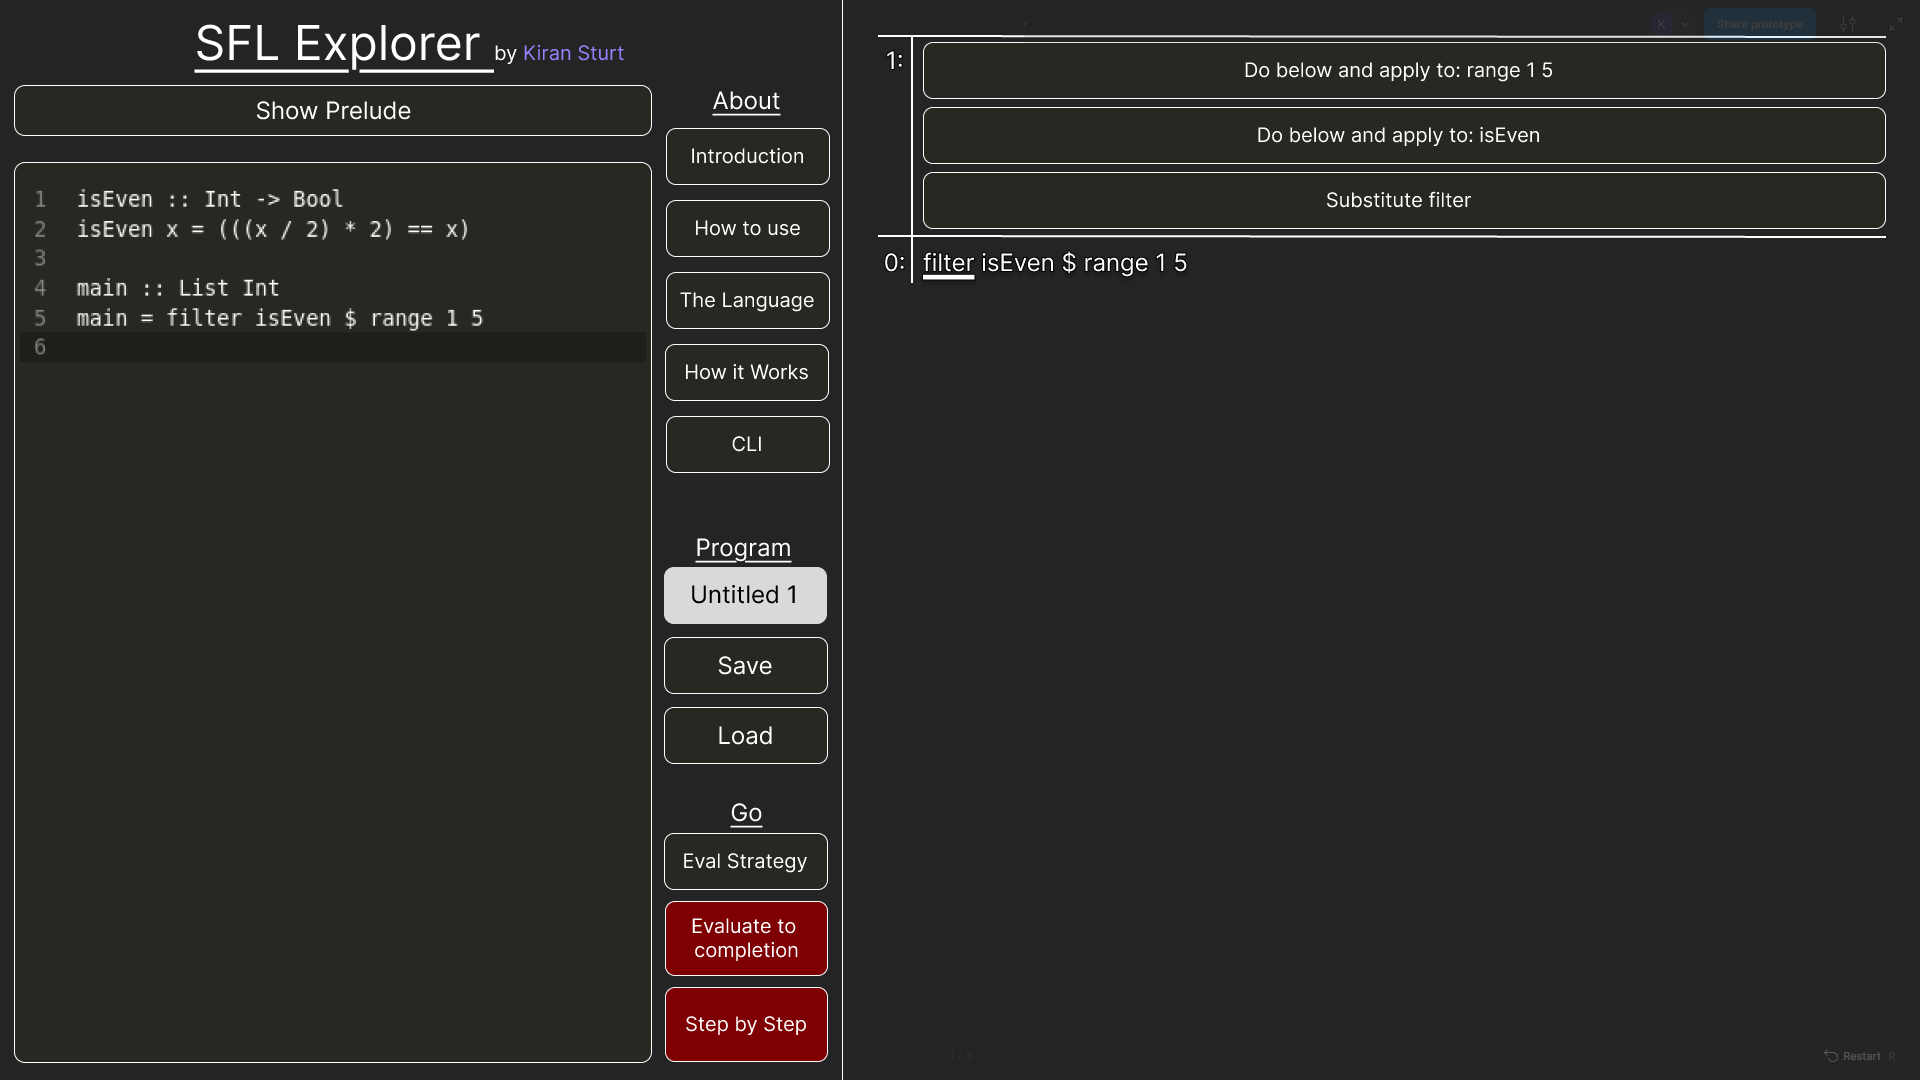
\includegraphics[width=1\linewidth]{images/figma_1.png} 
    \captionsetup{justification=centering}
    \caption{Screenshot 1 of the Figma design of the web UI\sam{formatting bug bear: put full stops at the end of captions}}
    \label{fig:screenshot_figma1}
\end{figure}

\begin{figure}[h]
    \centering
    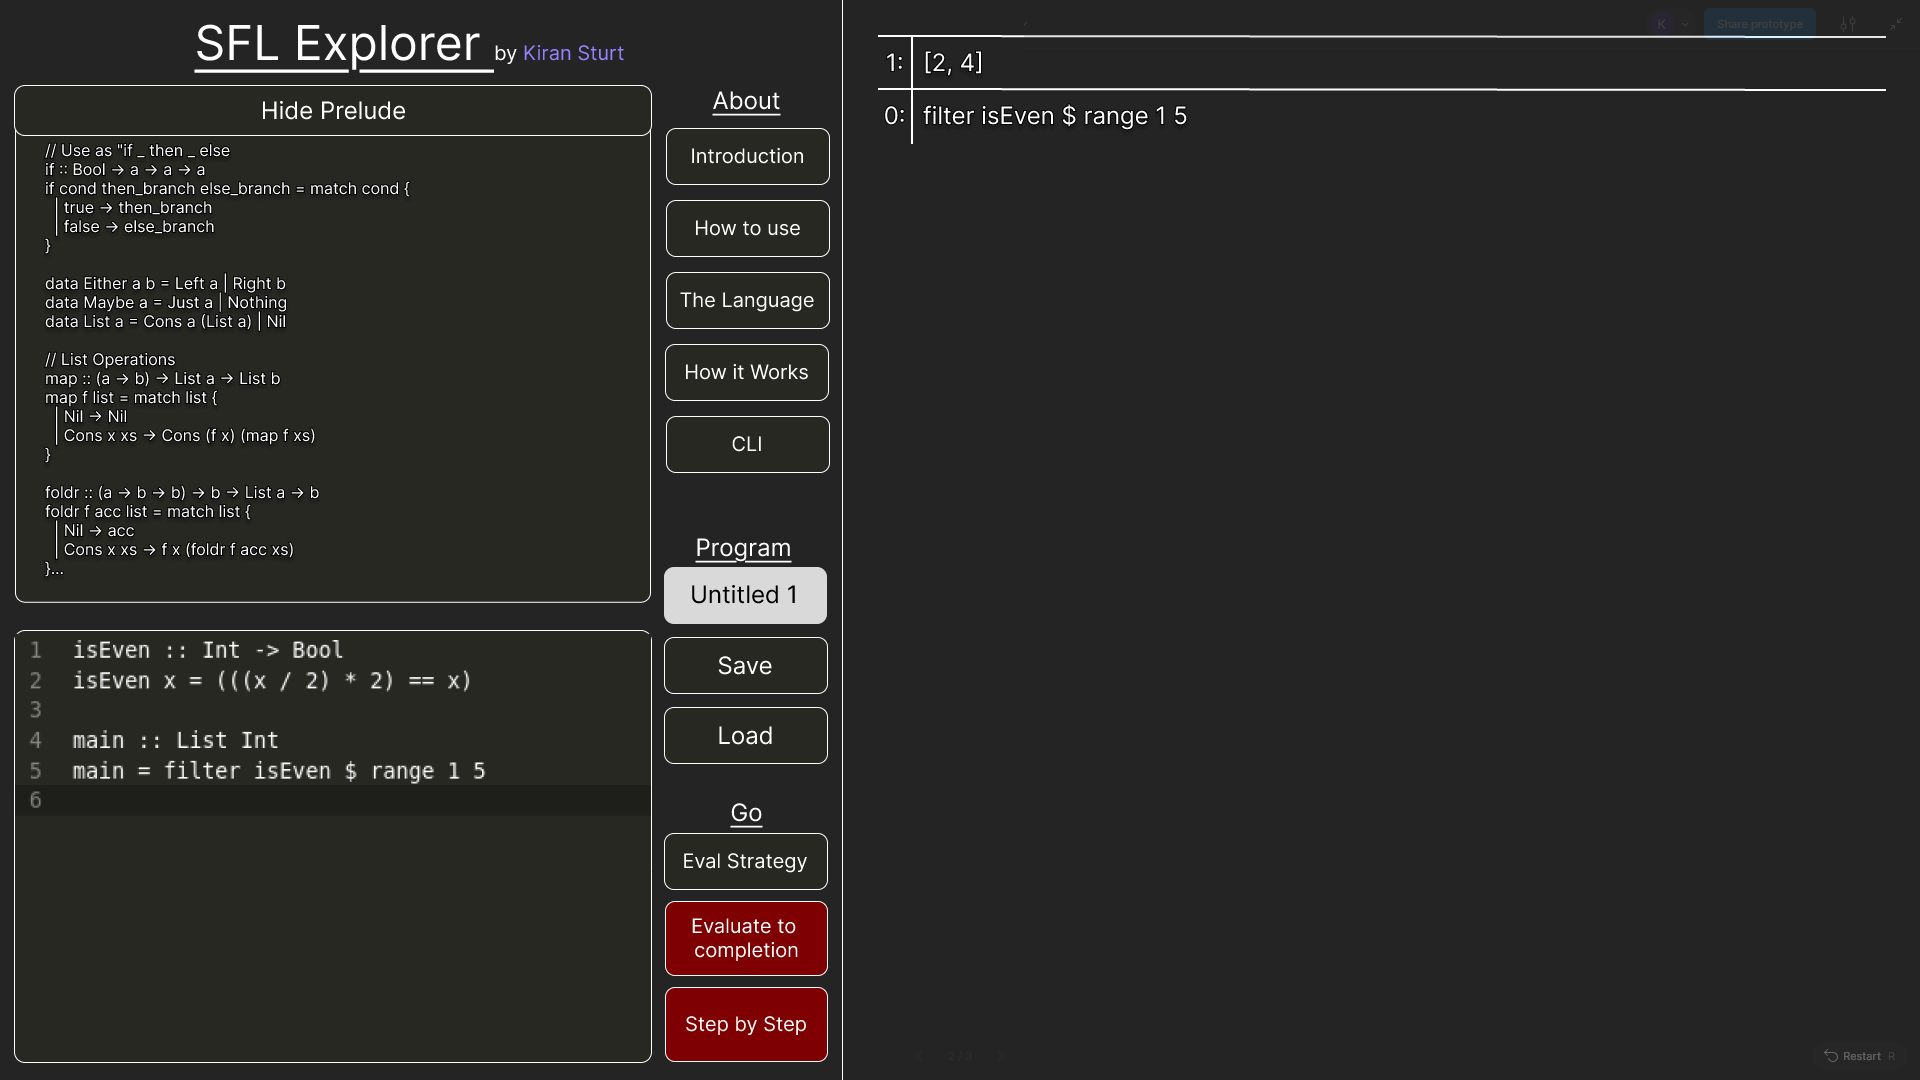
\includegraphics[width=1\linewidth]{images/figma_2.png}
    \captionsetup{justification=centering}
    \caption{Screenshot 2 of the Figma design of the web UI. This version shows the prelude extended \sam{here is motivation as to why, it looks like somethign following extended has been cut off}}
    \label{fig:screenshot_figma2}
\end{figure}

This design was meant to be a work in progress, but it looks quite similar to the final release of the product (Screenshots \ref{fig:screenshot_final_dark}, \ref{fig:screenshot_final_light}, \ref{fig:screenshot_final_dark_prelude_free} and \ref{fig:screenshot_final_light_prelude_free}). Before implementing this design, I discussed this design with the Advanced Focus Group (see \ref{ref:afg_figma}) and they were much more positive about this UI than the existing one 
\todo{Discuss revert}\\
\todo{Design principle: simplicity, speed, minimalism, feeling like vscode.}

\section{Implementation}

\subsection{Types}

Rust allows us to represent our types (see \ref{fig:tc_types} for the definition of the type system) quite easily using Enums. Rust's Enums are an example of algebraic data types, and are therefore very useful for defining our own algebraic data type system. See \ref{fig:type_lst} for the listing. 

\begin{figure}[ht]
    % \centering
    % \begin{tabular}{c}
    % \hline
    \begin{lstlisting}[language=Rust_boxed]
pub enum Primitive {
    Int64,
    Bool,
}

pub enum Type {
    Unit,
    Primitive(Primitive),
    Function(Box<Type>, Box<Type>),
    TypeVariable(String),
    Forall(String, Box<Type>),
    Product(Box<Type>, Box<Type>),
    Union(String, Vec<Type>),

    Alias(String, Box<Type>),
    Existential(usize),
}
\end{lstlisting}
    % \\\hline
    % \end{tabular}
    \caption{The Rust code listing for the definition of types. `Existential' and `Alias' are separated as they are more of an implementation detail than a part of the type system}
    \label{fig:type_lst}
\end{figure}

We must use \verb|Box<Type>|, which represents a pointer to a heap allocated object, otherwise it would be impossible to calculate the size of \verb|Type|, as it could be infinitely large with it containing another \verb|Type| recursively. \verb|Box<Type>| however has known size: the size of a pointer in the target architecture. 

We also define Existential, as an implementation detail needed for the type checker. 

Aliases are defined here with their name, and the type they are an alias for. Aliases could simply be implemented by replacing all occurrences of the string on the left with the string on the right, but defining them here allows us to use their names to generate type errors making them easier to understand. 

\subsubsection{Methods on Types}
Below are a selection of the more important or interesting methods implemented on Types.
\sam{didn't we have similar before?}

\paragraph{Substitution of type variables} \sam{it is annoying that para has the same formatting as subsubsection, if you have spare time, id change that as it makes reading harder}We may wish to set a type variable to another type. For instance, if given the type expression \(T \; U\) where \(T\) and \(U\) are types, and we know that one of the constructors of \(T\) is of generic type \(\forall a.a \rightarrow T \; a\), the type of the constructor for this type should be \(U \rightarrow T \; U\). We have `instantiated' the type variable \(a\) to be \(U\) by substituting \(a\) with \(U\) throughout the expression, and removing the \(\forall a\). This is required for the type checker. 

\paragraph{To String} We will frequently wish to display types as strings for debugging purposes. 
\subsection{Type Assignment and Definition Parsing}
We must also be able to parse type assignments (\verb|x :: Int|) and type definitions (\verb|type a|, or \verb|data a|). Parsing both of these things require the ability to parse type expressions. 

\subsubsection{Parsing Type Expressions}
Type expressions can be parsed using recursive descent parsing. Our connective for our parsing is arrow: `\verb|->|', and our primaries are anything that does not contain arrows. The structure of the type expression parser is similar to that of the expression parser. We first parse a primary, and then we terminate or parse our connective. The algorithm for parsing a primary is as follows:

\paragraph{Parsing Type Expression Primaries}
\begin{verbatim}
function parse_type_expression_primary(bound_type_variables, type_table) {
    next_token = consume()
    match (next_token) {
        case lowercase_id {
            name = next_token.value
            if bound_type_variables exists {
                if !bound_type_variables.contains(name) {Error}
            }
            return TypeVariable(name)
        }
        case uppercase_id {
            name = next_token.value
            if type_table.contains(name) {
                return type_table.get(name)
            } else {Error}
        }
        case left_paren {
            return parse_type_expression(bound_type_variables, type_table)
        }
        otherwise Error
    }
}
\end{verbatim}

\subsubsection{Parsing Type Alias Definitions} 
We may wish to add another name that a type can be known by. For instance, we may wish to define `\verb|String|' as a list of characters, so that we may reference it easier. A type alias declaration consists of:
\begin{itemize}
    \item The `\verb|type|' keyword
    \item The name of the alias
    \item The assignment operator ($=$)
    \item The type expression
\end{itemize}
The function that produces type aliases returns a `\verb|Type::Alias(String, Box<Type>)|'. The reason we do not want to simply rename all references to the alias name to the type in question is that this would make type errors more obscure, and harder for users to understand the error with reference to the original program.

\subsubsection{Parsing Data Declaration} 
As discussed in [REFHERE: Language Design], we want to be able to define and parse \verb|data| declarations. A \verb|data| deceleration consists of: 
\begin{itemize}
    \item The `\verb|data|' keyword
    \item The name of the type (uppercase ID)
    \item The assignment operator (=)
    \item A set of constructors separated by \(\mid\). Constructor definitions consist of the following. 
        \begin{itemize}
            \item The name of the constructor
            \item Zero or more type expressions, representing what types the constructor can be applied to.
        \end{itemize}
\end{itemize}

An example definition is: `\verb!data Either a b = Left a | Right b!'. The information that should be extracted from here is:
\begin{itemize}
    \item `\verb|Either|' is a type constructor with a kind of \(*\rightarrow* \rightarrow *\). As we have no higher kinded types, this can simply be stored as a number representing the arity of the type constructor. In this case, the arity is 2.
    \item The constructors and their types are:
    \begin{itemize}
        \item `\verb|Left|': \(\forall a\;b.a\rightarrow Either\;a\;b\)
        \item `\verb|Nil|': \(\forall a\;b.b\rightarrow Either\;a\;b\)
    \end{itemize}
\end{itemize}
We must store the type name and its arity in the `Type Table', and all constructors in the `Label Table'. 

In order to parse the type constructor definition, we continually expect a lowercase identifier token until we reach the assignment operator `\verb|=|'. The lowercase identifiers declared are passed to the functions that parse constructors so that we can enforce that all of the type variables used in the constructor parsing are `in scope'. We also do this to make sure that the variables are correct, and in the correct order in the constructor definitions. 

Parsing constructors is not complex, as we have already implemented the mechanism for parsing type expressions. We simply keep parsing expressions until either the constructor separator ($\mid$) or a newline is reached. When parsing the type expression, we expect only valid concrete types in the Type Table, or valid in scope type variables from the type constructor definition. We then produce a type from the types of the arguments in order, so `\verb|ConstructorName expr1 expr2 expr3|' results in the type `\(expr1  \rightarrow expr2 \rightarrow expr3 \rightarrow  TypeName\)', with all of the free type variables lifted to the start of the type into a series of nested `\verb|Type::Forall|'s.

\newpage
\subsection{The Type Checker}
The type checker will be bidirectional, and will follow an algorithm largely based on the one described by Dunfield and Krishnaswami \cite{completebidir}. The quote that follows from this paper, describes bidirectional type checking and its merits: \sam{another weird intro}
\begin{quote}
`Bidirectional typechecking, in which terms either synthesize a type or are checked against a known type, has become popular for its scalability \ldots its error reporting, and its relative ease of implementation' \cite{completebidir}
\end{quote}
\noindent It was the `relative ease of implementation' that attracted me to bidirectional type checking. I modified their algorithm to add my extra types (the inbuilt types $Int$, $Bool$, as well as the \Uniontype\ and \Producttype\ types) and my extra expression syntax structures (literals, match, pairs). This does not include assignment and modules as these are not part of expression syntax. 

\begin{figure}[h]
  \centering
  \begin{minipage}{\textwidth}
  \[
      \begin{array}{llcl}
      % \\[4pt]
      \text{Types} & A, B, C & \bnfas &
            \Inttype \bnfalt \Booltype \bnfalt \alpha \bnfalt \ahat \bnfalt 
            % \\[1pt] &&&\!\!\!\;\;\;
            \alltype{\alpha}{A} \bnfalt A \arr B \bnfalt
            % \\[1pt] &&&\!\!\!\;\; \TypeAlias{A}{B} \bnfalt  
            % \\[1pt] &&&\!\!\!\;\;
            (A, B) \bnfalt
            % \\[1pt] &&&\!\!\!\;\;
            \Unionname[A_1, \dots, A_n]
      \\[2pt]
      \text{Monotypes} & \tau,\sigma & \bnfas &
            \Inttype \bnfalt \Booltype \bnfalt \alpha \bnfalt \ahat \bnfalt 
            % \\[1pt] &&&\!\!\!\;\;
            \tau \arr \sigma \bnfalt (\tau, \sigma) \bnfalt \Unionname[\tau_1, \dots, \tau_n]
            % (A, B) \bnfalt \TypeAlias{A}{B}
        \\[2pt]
      \text{Contexts} & \Gamma, \Delta, \Theta & \bnfas &
                  \cdot
                  \bnfalt \Gamma, \alpha 
                  \bnfalt \Gamma, x:A
                  % \\[1pt] &&&\!\!\!\;\;
                  \bnfalt \Gamma, \ahat
                  \bnfalt \Gamma, \hypeq{\ahat}{\tau}
                  % \\[1pt] &&&\!\!\!\;\;
                  \bnfalt \Gamma, \MonnierComma{\ahat}
      % \\[2pt] % No need as I am not proving completeness
      % \text{Complete Contexts}     & \Omega & \bnfas &
      %             \cdot
      %             \bnfalt    \Omega, \alpha
      %             \bnfalt    \Omega, x:A
      %             \\[1pt] &&&\!\!\!
      %             \bnfalt    \Omega, \hypeq{\ahat}{\tau} 
      %             \bnfalt    \Omega, \MonnierComma{\ahat}
      \end{array}
  \]
  
  \captionsetup{justification=centering}\caption{Syntax of types, monotypes, and contexts as seen by the typechecker. The definition of types differ slightly from the definition offered in figure \ref{fig:sfl_types_no_exst}, as we include existential type variables ($\ahat$) that can not actually be created by users. They are an implementation detail required for the type checking algorithm}
  \FLabel{fig:tc_types}

  
  \end{minipage}
  \hfill
  \begin{minipage}{\textwidth}
    \centering
      \[
  \begin{array}[t]{l@{~}c@{~}ll}
      %
      [\Gamma]\Inttype  & = & \Inttype &\\{}

      [\Gamma]\Booltype & = & \Booltype &\\{}

      [\Gamma]\alpha    & = & \alpha &\\{}
      % [\Gamma]\unitty   & = &   \unitty &
      % \\[1pt]
      \big[\Gamma[\hypeq{\ahat}{\tau}]\big] \ahat
               & = &   \big[\Gamma[\hypeq{\ahat}{\tau}]\big]\tau &
      \\[2pt]
      \big[\Gamma[\ahat]\big]\ahat   & = &   \ahat &
      \\[2pt]
      [\Gamma](A \arr B)   & = &
          ([\Gamma]A) \arr ([\Gamma]B) &
      \\{}
      [\Gamma](\alltype{\alpha} A)
         & = & 
         \alltype{\alpha} [\Gamma]A &
      \\[2pt]
      [\Gamma](A, B) 
         & = &
         ([\Gamma]A, [\Gamma]B)
      \\[2pt]
      [\Gamma]\Unionname[A_1,\dots, A_n]
         & = &
         \Unionname[[\Gamma]A_1,\dots, [\Gamma]A_n]
  \end{array}
  \]
  \captionsetup{justification=centering}\caption{Applying a context, as a substitution, to a type}
  \FLabel{fig:ctx_subst}
  \end{minipage}
\end{figure}


% The full typechecking algorithm is listed in figures \ref{fig:alg-subtyping}, \ref{fig:instantiation}, \ref{fig:alg-typing}. 


\paragraph{Hole notation}
% \sam{you have not prepared the reader for this extract, I'll inline my questions to illustrate}
Below is a paragraph from the original paper \cite{completebidir} explaining `hole notation' in contexts, which is used throughout the algorithm descriptions in \ref{fig:alg-typing}, \ref{fig:alg-subtyping} and \ref{fig:instantiation}. 
\begin{quote}
`Since we will manipulate contexts not only by appending declarations \dots but by inserting and replacing declarations in the middle, a notation for contexts with a hole is useful:
\vspace{-4pt}
\begin{displ}
  `$\Gamma = \Gamma_0[\Theta]$~~~means $\Gamma$ has the form $(\Gamma_L, \Theta, \Gamma_R)$
\end{displ}
% \sam{where does $\Gamma_0$ go? where do $\Gamma_L$ and $\Gamma_R$ come from?}
For example, if $\Gamma = \Gamma_0[\bhat] = (\ahat, \bhat, x : \bhat)$,
then $\Gamma_0[\hypeq{\bhat}{\ahat}] = (\ahat, \hypeq{\bhat}{\ahat}, x : \bhat)$
% \sam{what is $\hypeq{\bhat}{\ahat}$ why are there two $\bhat$}
\newline\dots\newline
% \sam{...?}
% \sam{this is the most complex thing so far, here is where you need to spend your time, and start with an example}
% \sam{yes you are building on prev work, so your extensions are of most interest, but i cant appreciate them if i dont understand the base algo, also you must demo that you know the base algo}
Occasionally, we also need contexts with \emph{two} ordered holes:
\begin{displ}
  $\Gamma = \Gamma_0[\Theta_1][\Theta_2]$
  ~~~means
  $\Gamma$ has the form $(\Gamma_L, \Theta_1, \Gamma_M, \Theta_2, \Gamma_R)$' \cite{completebidir}
\end{displ}
\end{quote}

\noindent Below I will describe the typechecking algorithm, focusing on my additions/changes. Appendix \ref{appx:example_derive} shows some example derivations using this algorithm including some of my rules. 
% \sam{please run a small example inline here}
% \sam{you cannot rely on readers looking at your appendix}
% \sam{now i have read the appendix, It is excellent!!! just move that. Its so much clearer and its not dry cos we gave a goal and it nicely guides me through}

\subsubsection{Algorithmic Type Checking and Synthesis}
\begin{figure*}[t]
    \begin{minipage}{1\textwidth}
    \judgbox{\chkjudg{\Gamma}{e}{A}{\Delta}}%
    {Under input context $\Gamma$, $e$ checks against input type $A$, 
    with output context $\Delta$} \\[1ex]
 \judgbox{\synjudg{\Gamma}{e}{A}{\Delta}}%
    {Under input context $\Gamma$, $e$ synthesizes output type $A$,
      with output context $\Delta$} \\[0.5ex]
 \judgbox{\appjudg{\Gamma}{e}{A}{C}{\Delta}}%
    {Under input context $\Gamma$, applying a function of type $A$ to $e$ synthesizes type $C$, \\ with output context $\Delta$} \\
    \end{minipage}
    \noindent\rule{\textwidth}{0.4pt}
    \caption{Checking and Synthesis rule formatting as described by Dunfield and Krishnaswami \cite{completebidir}}
\end{figure*}

Figure \ref{fig:alg-typing} shows the main algorithm for checking and synthesizing the types of various expression structures. The rule I added are: 
%\sam{questions the reader might have: but how is this an algo? they are sequences of steps? What is all this notation? I've never seen the backwards turnstyle before or the backward implication. This should be walked thorugh in prose, you should not expect me to spend ages looking at the figure figuring it out. You are the writer, guide me}
%\sam{say in the prose that they are highlighted. I think the way you use captions is weird. It reads as if your expectation upon someone reading "figure bla" is that they immediately read the caption of figure  bla, but i dont. I stick with the prose hoping to be guided through my viewing of the figure, especially such a complex one.}
\begin{itemize}
    \item Checking and synthesizing rules for $Int$s and $Bool$s: An int literal synthesizes the type $Int$, and checks against the type $Int$ etc. 
    %\sam{there is a way to reference rules, which might be nice here}
    \item Checking and synthesis rules for pairs
    \begin{itemize}
        \item A pair $(e_1, e_2)$ checks against type $(A, B)$ if $e_1$ checks against $A$ and $e_2$ checks against $B$. 
        \item If $e_1$ synthesizes type $A$ and $e_2$ synthesizes type $B$ then $(e_1, e_2)$ synthesises $(A, B)$
    \end{itemize}
    \item The rule for synthesizing the type of a match expression. We synthesize the type of the expression being matched to a type $A$ (\synjudg{\Gamma}{e}{A}{\Delta}). We then check all the types of the patterns against type $A$. To get the output type, we add an existential type variable $\ahat$ to our context, and then check the type of all the output expressions against the type $\ahat$. We synthesize the type $\ahat$. The context is passed through all of these operations, and the final context contains all of the things `learned' from typechecking the match expression. 
    % \sam{this is better, but match each sentence to the symbols you are describing, I've inlined an example}
\end{itemize}

Note that the checking rules $\MyTCRule{\Intcheckrulename}$, $\MyTCRule{\Boolcheckrulename}$, $\MyTCRule{\Paircheckrulename}$ are not actually necessary, as they could be caught by the $\Sub$ rule. They are included as they remove the unnecessary steps that using the $\Sub$ rule in this manner creates, speeding up/simplifying the algorithm.

\subsubsection{Algorithmic Subtyping} \sam{you need an example} Figure \ref{fig:alg-subtyping} shows the algorithm for how we verify that a type is a subtype of another type. For instance, our typechecking rule $\Sub$ synthesizes the type, and the uses the algorithmic subtyping rules to check that the synthesized type is a subtype of the expected type. I have added rules for
\begin{itemize}
    \item $Int \subtype Int$ and $Bool \subtype Bool$ trivially. 
    \item $(A_1, B_1) \subtype (A_2, B_2)$ if $A_1 \subtype A_2$ and $B_1 \subtype B_2$.
    \item The union with name $N_1$ and arguments $A_1 \dots A_n$ is a subtype of a union with name $N_2$ and arguments $B_1 \dots B_n$ is a subtype, if the names are the same as the names uniquely identify these types, as well as all the constituent types being subtypes of each other. The context is passed through all of these operations, and the final context contains all of the things `learned' from typechecking the match expression.
\end{itemize}

\subsubsection{Context Instantiation} 
Figure \ref{fig:instantiation} shows the special subtyping rules for existential type variables that also instantiates the variable within the context. The subtyping rule $\SubInstL$ allows us to derive that the existential type variable $\ahat$ is a subtype of the type $A$. It requires that we instantiate $\ahat$ to the value of $A$ in our context. $\SubInstR$ does the opposite. Both add to the context all the information we gain about $\ahat$ by saying that it is a subtype of $A$, or that $A$ is a subtype of it. 

For instance, the rule $\InstLArr$ instantiates $\ahat$ such that $\ahat \subtype A_1 \arr A_2$ by adding to our context $\ahat_1, \ahat_2$, and setting $\ahat = \ahat_1 \fto \ahat_2$ in the context. We then instantiate $\ahat_1 \instsymlop A_1$ and $\ahat_2 \instsymrop A_2$.

\subsubsection{Typechecking the Pair Function}
This is an example of the algorithm in action. The pair function $\lam{x\;y} (x, y)$ takes two arguments, and returns a pair of the two values. Here, we type check it against its correct type $\alltype{\alpha\;\beta}{\alpha \fto \beta \fto (\alpha, \beta)}$. Type checking/synthesis is done recursively from bottom up, so read [1] upwards. 

\begin{mathpar}
\Gamma = \alpha,\beta,x : \alpha,y : \beta\\
\Delta = \alpha\\

\Infer{\Sub[6]}
  {\Infer{\Var[8]}
      {(x : \alpha) \in \{\Gamma\}}
      {\synjudg{\Gamma}{x}{\alpha}{\Gamma}}
    \\
  \Infer{\SubVar[9]}
      { }
      {\subjudg{\Gamma[\alpha]}{\alpha}{\alpha}{\Gamma[\alpha]}}
  }
  {\chkjudg{\Gamma}{x}{\alpha}{\Gamma}}
\\

\Infer{\Sub[7]}
  {\Infer{\Var[10]}
      {(y : \beta) \in \{\Gamma\}}
      {\synjudg{\Gamma}{y}{\beta}{\Gamma}}
    \\
  \Infer{\SubVar[11]}
      { }
      {\subjudg{\Gamma[\beta]}{\beta}{\beta}{\Gamma[\beta]}}
  }
  {\chkjudg{\Gamma}{y}{\beta}{\Gamma}}

 \Infer{\AllIntro[1]}
   {\Infer{\AllIntro[2]}
   {
    \Infer{\!\ArrIntro[3]}
      {
       \Infer{\!\ArrIntro[4]}
          {
          \Infer{\MyTCRule{\Paircheckrulename}[5]}
            {[6]\chkjudg{\Gamma}{x}{\alpha}{\Gamma} \\ [7]\chkjudg{\Gamma}{y}{\beta}{\Gamma}}
            {\chkjudg{\Gamma}{(x, y)}{(\alpha, \beta)}{\Gamma}}
          }
          {\chkjudg{\alpha,\beta,x : \alpha}{\lam{y} (x, y)}{\beta \fto (\alpha, \beta)}{\Gamma}}
          }
      {{\chkjudg{\alpha,\beta}{\lam{x\; y} (x, y)}{\alpha \fto \beta \fto (\alpha, \beta)}{\Delta, \beta, \{x : \alpha, y : \beta\}}} \\ (= \Gamma)}
   }
   {{\chkjudg{\alpha}{\lam{x\;y} (x, y)}{\alltype{\beta}{\alpha \fto \beta \fto (\alpha, \beta)}}{\{.\}, \alpha, \{.\}}} \\ (= \Delta)}
   }
   {\chkjudg{.}{\lam{x\;y} (x, y)}{\alltype{\alpha\;\beta}{\alpha \fto \beta \fto (\alpha, \beta)}}{.}}\\

\end{mathpar}

\begin{enumerate}
    \item Here, we begin typechecking with the \AllIntro rule to introduce $\forall \alpha$. We do this by adding $\alpha$ to the initially empty context. We then check the function against the type without the $\forall \alpha$: $\alltype{\beta}{\alpha \fto \beta \fto (\alpha, \beta)}$. The output of this checking is then split into 3 parts: everything before the $\alpha$, the $\alpha$ itself, and the bits after the $\alpha$. Our output context is everything in $\Delta$ before the alpha, which is nothing. 
    \item We apply the same rule as above, but we are introducing $\forall \beta$. We then check the function against ${\alpha \fto \beta \fto (\alpha, \beta)}$
    Our output context for this rule is everything in $\Gamma$ before the $\beta$: only $\alpha$.
    \item We then start to unwrap the abstractions. We strip the abstraction over $x$ from the expression, leaving us with ($\lam{y} (x, y)$). We then add $(x:\alpha)$ to our context, and then progress by checking the remaining part of the expression against ${\beta \fto (\alpha, \beta)}$. Our output context is $\Gamma$. 
    \item Same as above, with $y$ against $\beta$. We unwrap the abstraction over $y$ to give us $(x, y)$. We then check this against ${(\alpha, \beta)}$. The output context is $\Gamma$.
    \item We check $(x, y)$ against the type $(\alpha, \beta)$. To check this, we check $x$ against $\alpha$ and $y$ against $\beta$. The output context is $\Gamma$.
    \item To check $x$ against type $\alpha$ we synthesise the type of $x$ ([9]: trivial, as its in the context). We then check this against $\alpha$, and a check of $\alpha$ against $\alpha$ ([10]) trivially passes.
    \item Same as above with $y$ against $\beta$. The output context is $\Gamma$
\end{enumerate}


\subsection{Synthesizing Example}
We have a function \sflinline{f x = Just x} (desugared: \sflinline{f = (\x. Just x)}) that we want to synthesize the type of. \sflinline{Just} is a constructor defined in the type declaration \sflinline{data Maybe a = Just a | Nothing}, and it has a type $\forall a. a \arr Maybe\,a$

\begin{mathpar}
T_{Just} = \forall \alpha. \alpha \arr \textit{Maybe}\,\alpha \and
T_{Nothing} = \forall \alpha. \textit{Maybe}\,\alpha \\
\Gamma_0 = Just: T_{Just},\; Nothing: T_{Nothing}\and
\Gamma_1 = \Gamma_0, \ahat, \bhat, x : \ahat\and
\Gamma_2 = \Gamma_1, \chat \\
\Gamma_3 = \Gamma_1, \hypeq{\chat}{\ahat} \and
\Gamma_4 = \Gamma_0, \ahat, \hypeq{\bhat}{\textit{Maybe}\,\ahat}, x : \ahat, \hypeq{\chat}{\ahat}\\

\Infer{\InstRSolve[12]}
{\Gamma_3 \entails \textit{Mabye}\,\ahat}
    {\instjudgr{\{\Gamma_0, \ahat\}, \bhat, \{x : \ahat, \hypeq{\chat}{\ahat}\}}
        {\bhat}
        {\textit{Mabye}\,\ahat}
        \{{\Gamma_0, \ahat\}, \hypeq{\bhat}{\textit{Mabye}\,\ahat}, \{x : \ahat, \hypeq{\chat}{\ahat}\}}
    }\\


\Infer{\SubInstR[11]}
{
    \bhat \notin \FV{%
    \textit{Mabye}\,\ahat}
    \\
    {\instjudgr{\Gamma_3}
        {\bhat}
        {\textit{Mabye}\,\ahat}
        {\Gamma_4}} [12]
}
{\subjudg{\Gamma_3}{\textit{Mabye}\,\ahat}{\bhat}{\Gamma_4}}\\



\Infer{\SubInstL[9]}
{
    \ahat \notin \FV{%
        \chat}
    \\
    \Infer{\InstLReach[10]}
    { }
    {\instjudg{\Gamma_2[\ahat][\chat]}
            {\ahat}
            {\chat}
            {\Gamma_2[\ahat][\hypeq{\chat}{\ahat}]}}
}
{\subjudg{\Gamma_2}{\ahat}{\chat}{\Gamma_3}} \\

\Infer{\ArrApp[6]}
{
    \Infer{\Sub[7]}
        {
            \Infer{\Var[8]}
                {(x : \ahat) \in \Gamma_2}
                {\synjudg{\Gamma_2}{x}{\ahat}{\Gamma_2}}
            \\
            \subjudg{\Gamma_2}{[\Gamma_2]\ahat}{[\Gamma_2]\chat}{\Gamma_3}\;\; [9]
        }
        {\chkjudg{\Gamma_2}{x}{\chat}{\Gamma_3}}
}
{\appjudg{\Gamma_2}{x}{\chat \arr \textit{Mabye}\,\chat}{\textit{Mabye}\,\chat}{\Gamma_3}} \\

\Infer{\!\ArrElim[3]}
    {\Infer{\Var[4]}
        {(Just : T_{Just}) \in \Gamma_1}
        {\synjudg{\Gamma_1}{Just}{T_{Just}}{\Gamma_1}}
        \\
        \Infer{\AllApp[5]}
            {\appjudg{\Gamma_1,\chat}{x}{[\chat/\alpha] (\alpha \arr \textit{Mabye}\,\alpha)}{\textit{Mabye}\,\chat}{\Gamma_3}[6]}
            {\appjudg{\Gamma_1}{x}{\alltype{\alpha}{\alpha \arr \textit{Mabye}\,\alpha}}{\textit{Mabye}\,\chat}{\Gamma_3}}
    }
    {\synjudg{\Gamma_1}{\textit{Just x}}{\textit{Mabye}\,\chat}{\Gamma_3}} \\

\Infer{%
{\!\ArrIntroSyn[1]}
    }
    { 
    \Infer{\Sub[2]}
    {
        \synjudg{\Gamma_1}{\textit{Just x}}{\textit{Mabye}\,\chat}{\Gamma_3}[3]
        \\
        \subjudg{\Gamma_3}{[\Gamma_3]\textit{Mabye}\,\chat}{[\Gamma_3]\bhat}{\Gamma_4}[11]
    }
    {\chkjudg{\Gamma_0, \ahat, \bhat, x : \ahat}{\textit{Just x}}{\bhat}{\{\Gamma_0, \ahat, \hypeq{\bhat}{\textit{Mabye}\,\ahat}\}, x : \ahat, \{\hypeq{\chat}{\ahat}\}}}
    % \chkjudg{\Gamma_0, \ahat, \bhat, x : \ahat}{\text{Just x}}{\bhat}{\{\Gamma_0, \ahat, 
    % \hypeq{\bhat}{Maybe\,\ahat}\}, x : \ahat, \{\hypeq{\chat}{\ahat}\}}
    }
    {{\synjudg{\Gamma_0}{\lam{x} \textit{Just x}}{\ahat \arr \bhat}{\Gamma_0, \ahat, \hypeq{\bhat}{\textit{Mabye}\,\ahat}}}} \\

\end{mathpar}

\begin{enumerate}
    \item We begin synthesis with the \ArrIntroSyn\ rule. We are trying to synthesize a type $A \arr B$  as the abstraction $\lam{x} \textit{Just x}$ must have a function type. We add to our context $\Gamma_0$ two existential type variables $\ahat, \bhat$. We also add to our context the type assignment $x: \ahat$, and then we check the inner body of the abstraction ($\textit{Just x}$) against $\bhat$ [1]. Check [1] yields the context $\Gamma_4$, and we discard everything after $x: \ahat$ to remove data we no longer need. We synthesize $\lam{x} \textit{Just x} \syn \ahat \arr \bhat$. Substituting the information from our context $\Gamma_4$ gives us $\ahat \arr \textit{Mabye}\,\ahat$. This is the final result of inference, but an existential type variables are simply a statement that `there exists a type', so they can be replaced with `$\forall$'s, giving our final result as $\forall a. a \arr \textit{Maybe}\,a$.
    % \addtocounter{enumi}{1}
    \item To check $\textit{Just x}$ against $\bhat$, we synthesize $\textit{Just x} \syn \textit{Mabye}\,\chat$ [3]. After applying $\Gamma_3$ as a substitution to $\textit{Mabye}\,\chat$ yielding $\textit{Mabye}\,\ahat$, we check this type against $\bhat$ [11], yielding $\Gamma_4$. 
    \item To synthesize the type of $\textit{Just x}$, we synthesize $\textit{Just} \syn T_{Just}$ [4], and synthesize the type of the application of type $T_{Just}$ to $\textit{x}$.
    \item From the context: $\textit{Just} \syn T_{Just}$
    \item To synthesize the type of applying $\forall \alpha. \alpha \arr \textit{Maybe}\,\alpha$ to $\textit{x}$, we unwrap the forall by substituting all of the $\alpha$s for a fresh existential type variable $\chat$. We then synthesisze the type of the application of $\chat \arr \textit{Maybe}\,\chat$ to $x$.
    \item To synthesisze the type of the application of $\chat \arr \textit{Maybe}\,\chat$ to $x$, we check $x$ against the first part of the arrow type $\chat$ [7]. We then yield the second part of the arrow type $\textit{Maybe}\,\chat$. 
    \item To check $x$ against $\chat$, we synthesize $x \syn \ahat$ [8], and then check that $\ahat \subtype \chat$ [9].
    \item From the context: $\textit{x} \syn \ahat$.
    \item We use the \SubInstL\ rule to derive $\ahat \subtype \chat$. We could have equally used \SubInstR\ as both rules are for deriving a subtyping judgement where one side is an existential, but here both are existentials. To do this, we check that $\chat$ has no free instances of $\ahat$, and we instantiate $\ahat$ such that $\ahat \subtype \chat$ [10].
    \item We instantiate $\ahat$ in our context $\Gamma_2$ to be a subtype of $\chat$ by setting $\chat$ to $\ahat$ in our context, yielding $\Gamma_3$.
    \item To check that $\textit{Maybe}\,a \subtype \bhat$, we check that $\textit{Maybe}\,a$ has no free instances of $\bhat$, and we instantiate $\bhat$ such that $\textit{Maybe}\,a \subtype \bhat$ [12].
    \item To instantiate $\bhat$ such that $\textit{Maybe}\,a \subtype \bhat$, we use the rule \InstRSolve\ to `solve' type $\bhat$ to be $\textit{Maybe}\,a$. This only requires that $\textit{Maybe}\,a$ is well formed under the context, which means that the context `knows about` all of the existential type variables (see \ref{fig:well_formed}).
\end{enumerate}

\subsection{Pairs}
To support pairs, we must first add `Pair' as an option to our enum `\verb|ASTNodeType|' \ref{fig:ast_lst}. A `Pair' node has \verb|ASTNodeType| of `Pair', and two children.

\subsubsection{Parsing Pairs}
Parsing pairs is trivial:
\begin{itemize}
    \item Expect an open parenthesis \verb|(|.
    \item Parse an expression.
    \item Expect a comma.
    \item Parse a second expression.
    \item Expect a closing parenthesis \verb|)|.
\end{itemize}
\noindent We then produce a `\verb|Pair|' \ac{AST} node with two children: the two expressions.
\subsubsection{Updating the Redex Finding System With Pairs}
Pairs themselves can never be redexes, so getting a list of all redex-contraction pairs in a `Pair' is trivial: we concatenate the list of \verb|RCPairs| in the left and right expression.

\subsection{Pattern Matching}
We add `Match' as an option to our enum `\verb|ASTNodeType|' \ref{fig:ast_lst}. A match node has many children. The first node represents the expression being matched over, then each case followed by its corresponding definition.
 
\subsubsection{Parsing Match Statements}
An example of using a match statement follows:
% \sam{here it feels like you are trying to mix up the way you introduce code so it is not always the same, but instead you have just ended up with a weird sounding sentence. It doesnt matter if introducing code uses the same phrasing, as long as it is clear.}
% \sam{more writing advice: only spend effort on nice writing for what is important. Introducing code not important, just do the basic thing. Biggest most complicated thing in your thesis is what deserves all your word choice and imagery. If you do this, it is also clear to the reader what is important: it is what you have spent your time on}
\begin{lstlisting}[language=SFL]
lengthIsAtLeast2 list = match list {
  | Cons x (Cons y xs) -> true
  | _ => false
}
\end{lstlisting}

The algorithm used for parsing match statements is:
\begin{enumerate}
    \item Consume the `match' keyword.
    \item Parse the expression matched over.
    \item Consume an open brace.
    \item While the next token isn't a close brace: \begin{enumerate}
        \item Consume bar `|'.
        \item Parse a pattern (\ref{impl:parsing_patterns}).
        \item Consume a right arrow.
        \item Parse an expression.
    \end{enumerate}
    \item Consume a close brace.
\end{enumerate}
This creates a `match' node, where the \verb|children| vector is set appropriately with the pattern and expressions.

\paragraph{Patterns}
\label{impl:parsing_patterns}
A pattern must not contain anything that can be reduced. It would be nonsensical to have a situation where we had a pattern not in normal form such as \verb|1 + 1| and the expression to be matched was \verb|2|. 

To parse a pattern, we may use the same techniques as parsing an expression, with a few differences:
\begin{itemize}
    \item Disallowing abstractions and match statements
    \item Identifiers must be either
    \begin{itemize}
        \item Unbound lowercase variables
        \item Underscore (\verb|_|) representing a wildcard pattern
        \item A bound uppercase variable (a constructor)
    \end{itemize}
\end{itemize}

\subsubsection{Updating the Redex Finding System With Pattern Matching}
As discussed in the design (\ref{c2_design_match}), patterns are checked in order from first to last. Not only do we need to check that it does not currently match before moving on to checking the next pattern, we must check that it \textit{can not} match the expression i.e. we must refute the pattern. In the below example, \sflinline{repeat 1} must be evaluated enough to know whether it matches the first pattern before we move on to matching the second. 

\begin{lstlisting}[language=SFL]
repeat :: a -> List a
repeat n = Cons n $ repeat n

main :: Bool
main = match repeat 1 {
    | Cons _ (Cons _ _) -> true
    | _ -> false
}
\end{lstlisting}

When matching an expression against a pattern, we have three possible results:

\begin{itemize}
    \item Success: Matching was successful, and we have a list of what to bind
    \item Refute: We can not match this pattern, and evaluating the expression further would definitely not result in being able to match
    \item Unknown: It does not match, but we cannot refute
\end{itemize}

The algorithm for finding the next evaluation step for a match expression is to sequentially attempt to match each pattern. If the result of matching an expression is a refutation, we check the next one. If the result is not yet known, we do not look at any further patterns, and we evaluate the expression further instead. 

Below is a short summary of how pattern matching is done for different structures. This summary does not show all cases, but instead aims to give a general idea about how the algorithm works. To match an expression $E$ against a pattern $P$ and get all variables that the pattern would bind, we proceed case wise on the structure of $P$. 
\begin{itemize}
    \item An Identifier \ref{fig:pattern_list_id}. 
    \begin{itemize}
        \item If the identifier is a lowercase variable, we succeed matching and returning the binding.
        \item If it is an underscore, matching succeeds, but we do not bind anything. 
        \item If it is an uppercase identifier (and therefore a constructor), we attempt to refute the pattern by showing that our expression will never evaluate to this constructor. Otherwise, our result is `unknown'.
    \end{itemize}

    % \item A pair: \ref{fig:pattern_list_pair}. We proceed case wise on the structure of $E$:
    % \begin{itemize}
    %     \item Another pair: we attempt to match the left and right of both pairs. If either Refutes then Refute, and if either is Unknown then return Unknown.
    %     \item Literal, Abstraction or Uppercase Identifier: Refute.
    %     \item Lowercase Identifier: Unknown, as it may stand for an expression that does evaluate to a pair
    % \end{itemize}
    
    \item An application: \ref{fig:pattern_list_app}. We proceed case wise on the structure of $E$:
    \begin{itemize}
        \item Literal, Pair, Abstraction or Uppercase Identifier: Refute as these will not evaluate further.
        \item Another application: Match the functions and match the arguments. If either Refutes then Refute, and if either is Unknown then return Unknown. Otherwise, Succeed, and concatenate the two lists of bindings
    \end{itemize} 

    \item A literal: trivial, the algorithm is just a string match. It is listed inline in \ref{fig:pattern_list_top_level} for completeness's sake. 
\end{itemize}

The algorithm for matching an expression against a single pattern, and getting either `Success, Refute, or Unknown' is listed in pseudocode: \ref{fig:pattern_list_top_level}. The algorithm for getting a redex-contraction pair from a match statement is also listed \ref{fig:all_pattern_list_iterate}. If we succeed in pattern matching, the result should be the appropriate case with all  the bindings substituted. 

\subsection{Multi Step Reduction and Lazy Mode}
As it currently stands, the system gives users the option to select any possible redex to make progress. However, whilst demonstrating this project to my client, I found that these steps were often too small, and sometimes one larger step would have been easier. I found that having to apply a nested abstraction to concurrent terms particularly tedious. The expression \sflinline{f 1 2 3} where \sflinline{f = (\x y z. x)} would have reduction sequence:
\begin{figure} %to avoid splitting 
\begin{itemize}
    \item \sflinline{f 1 2 3} \arr\ \verb|(\x y z. x) 1 2 3|
    \item \verb|(\x y z. 1) 1 2 3| \arr\ \verb|(\y z. 1) 2 3|
    \item \verb|(\y z. 1) 2 3| \arr\ \verb|(\z. 1) 3|
    \item \verb|(\z. 1) 3| \arr\ \sflinline{1}
\end{itemize}
\end{figure}
\noindent Many users of the system, particularly more advanced users, would not need to see each nested step of this application. These can all be grouped into one step, where we substitute label f and perform all three reductions simultaneously. 

\todo{Algorithm if time, and reformat reduction}

Users may not always want to choose reduction order themselves. The `Lazy' strategy \ref{bg:eval_strategies} is the one employed by Haskell and other functional languages, so it should be the one employed by \ac{SFL}. Conveniently, because of the way we are currently generating redexes, the list of redexes we generate already has the laziest option as the first element. This is because when generating redexes in an application, we calculate the redexes in the function before the redexes in the argument, which leads to a `leftmost first' list of redexes. 

\subsection{The Prelude, and `if e then a else b'}
Most programming languages come with functionality packaged that is included by default, and is written in the language. In Haskell, this is referred to as the Prelude. There is also the standard library which is more extensive and is not imported by default. 

As our language does not need extensive extra functionality, we do not need a whole standard library. However, a basic prelude with common functionality would be useful. \ref{appx:prelude} shows the SFL prelude. I included `if' in the prelude to show that it is based on a match statement, rather than being a mysterious inbuilt: 

\begin{lstlisting}[language=SFL]
if :: Bool -> a -> a -> a
if cond then_branch else_branch = match cond {
    | true -> then_branch
    | false -> else_branch
}    
\end{lstlisting}

In order to make the language more like Haskell, I also added syntax sugar that allowed you to use it using the `\lstinline[language=SFL_ite]|if e then a else b|' syntax. The parser would ignore the `\lstinline[language=SFL_ite]|then|' and the `\lstinline[language=SFL_ite]|else|' keywords, and it would be equivalent to `\lstinline[language=SFL_ite]|(((if e)  a)  b)|' internally. However, this was unpopular with the advanced focus group, who said that this was confusing (see \ref{ref:afg_ite}). 

The prelude is listed in the appendix: \ref{appx:prelude}.

\begin{figure}[h]
    \centering
    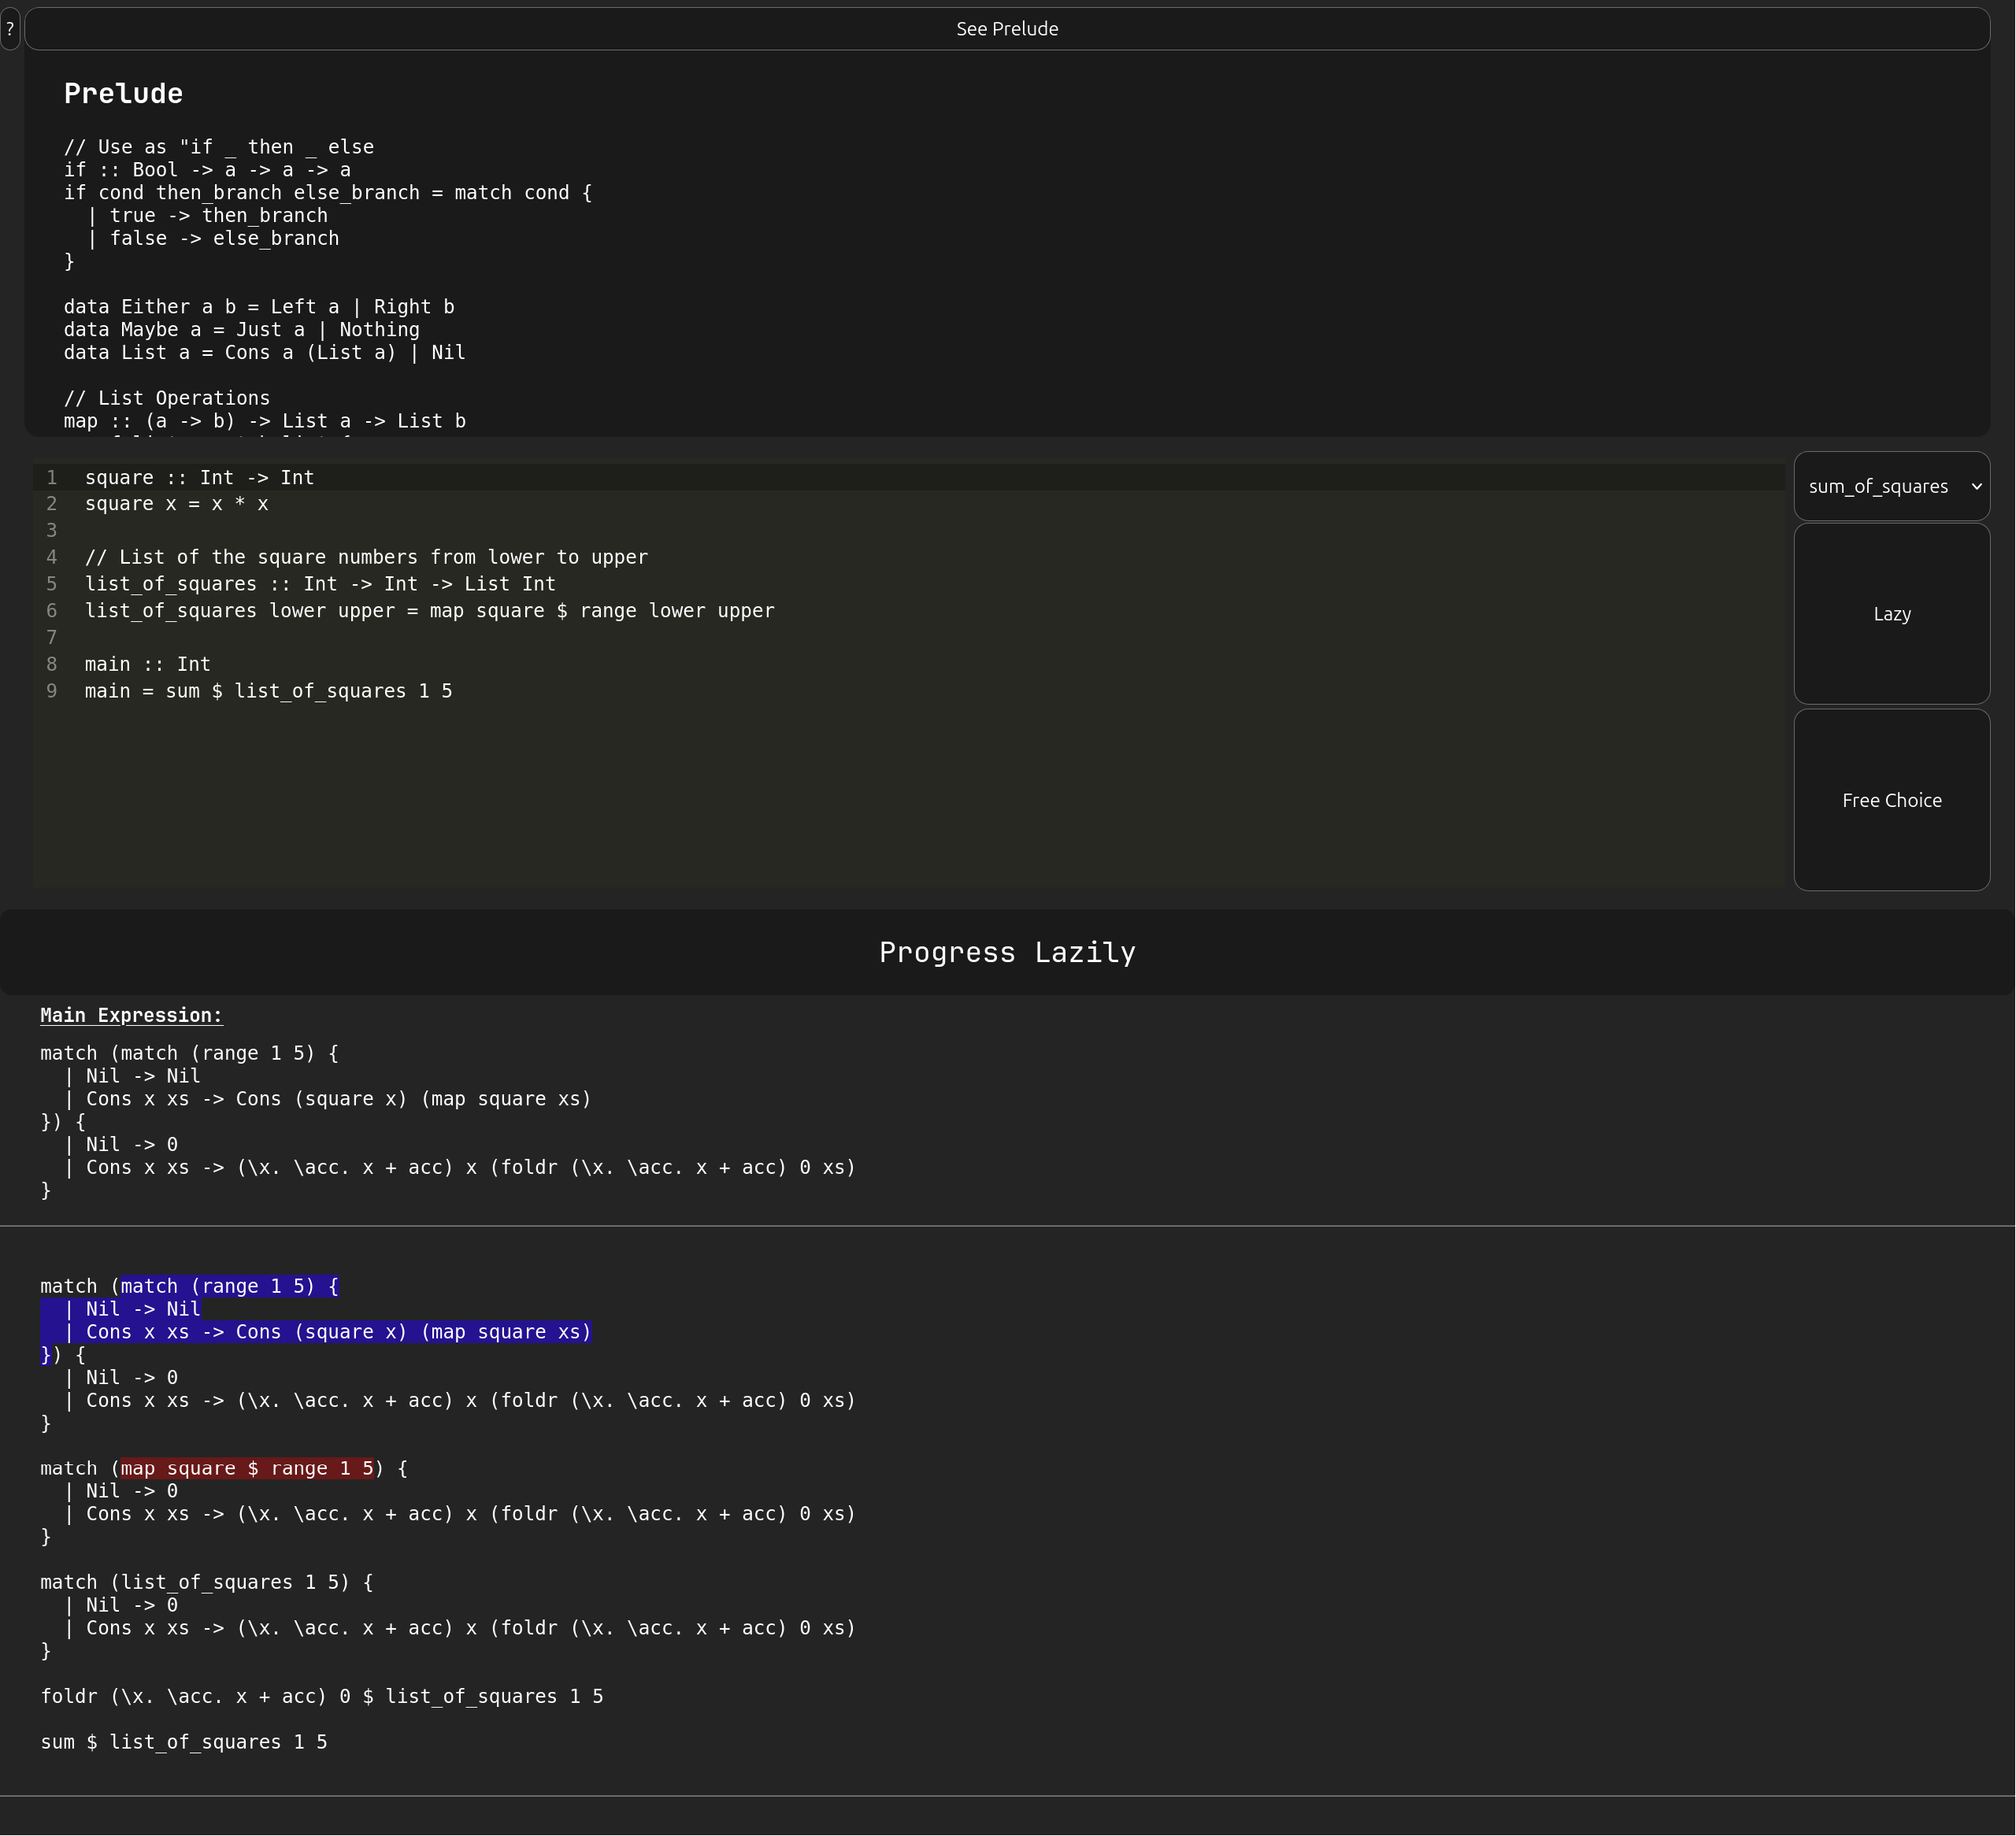
\includegraphics[width=1\linewidth]{images/phase-2-end2.png} 
    \captionsetup{justification=centering}
    \caption{The product at the end of phase two during lazy evaluation of the `sum of squares' sample program, with the prelude dropdown extended}
    \label{fig:screenshot_c2_end}
\end{figure}


\subsection{Changes to the Proof of Concept UI}
\label{c2_poc_ui_impl}
In this phase, I made some changes to the proof of concept web UI. See \ref{fig:screenshot_c2_end} and \ref{fig:screenshot_c2_end_free} for the desktop UIs, and \ref{fig:screenshot_phase2_mobile} for the mobile UI. 

\paragraph{Lazy Mode}
Added a separate `Lazy mode' which would only offer one button labelled `Progress Lazily'. The original functionality was included in `Free Choice' mode

\paragraph{History}
The history of the main expression is listed. The top two rows shows the most recent change, in blue is the result of the most recent change, in red is what it used to be. This does not work using the diff algorithm discussed in Phase 3 (\ref{paragraph:diff}), it instead gets the string before and the string after, and locates them in the second most recent and most recent program state. This is not fully accurate, as a string match results in false positives. If we reduced \sflinline{1 + 1} to \sflinline{2} in the expression \sflinline{(\x. x + (1 + 1)) (1 + 1)}, it would highlight both \sflinline{(1 + 1)}s even though the one in the abstraction has not been reduced. 

\paragraph{Other}

\begin{itemize}
    \item The prelude was offered as a dropdown.
    \item Some example programs can be loaded from a dropdown.  
    \item The program is saved in the browsers `localStorage' as it is edited
    \item A help menu was offered when the page was loaded, or when the `?' button in the top left corner was pressed: \ref{fig:screenshot_phase2_help}
\end{itemize}

\section{Testathon}
The testathon was a valuable opportunity to test my system at the midpoint of the project. During the testathon, I encouraged people to test the system on my laptop, as well as providing a QR code for them to be able to access it on their phone. I initially wanted to adopt a `think aloud' method for usability testing, which is `a method for studying mental process in which participants are asked to make spoken comment as they work on a task'\cite{thinkaloud}

The plan was to implement this, and passively watch them interact with the system and not give them any extra instruction. However, I found that people required significant instruction. I attempted to delegate any instruction to the `help menu', but this did not solve the problem for the following reasons: people do not naturally want to read instructions, and my instructions were insufficient for people asked to interact with the system without any guidance to be able to effectively use it. Many people couldn't find the instructions, or were confused by the notation.

\subsubsection{Data Gathering}
After I explained the system and participants engaged with the system, participants were asked to fill out a survey. There were 15 participants, who were a mixture of undergraduate and postgraduate computer scientists, all of whom had taken the first year \ac{FP} unit. 

% In one section of the survey, they were presented with a series of statements designed to gauge their feelings towards functional and imperative languages. A Likert scale\cite{likert1932technique} was used to measure the attitudes of participants towards the statements. See \ref{fig:imp_is_easy} for imperative results, and \ref{fig:fp_is_hard} for functional results. 

% \begin{figure*}[ht]
%     \begin{subfigure}{\textwidth}
%         \centering
%         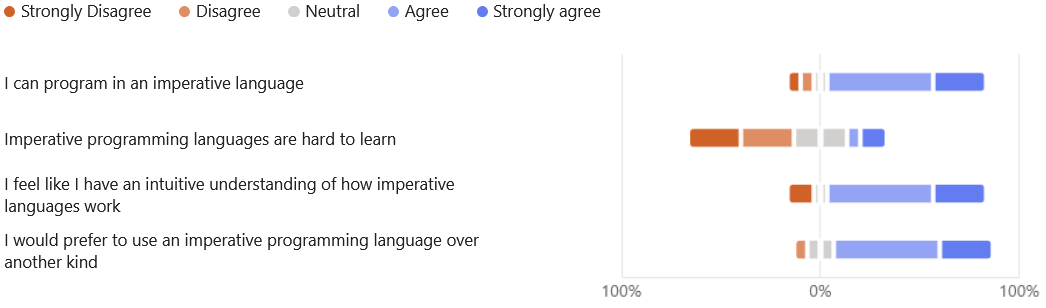
\includegraphics[width=\linewidth]{images/imperative_likert.png}
%         \caption{}
%         \label{fig:imp_is_easy}
%     \end{subfigure}
    
%     \begin{subfigure}{\textwidth}
%         \centering
%         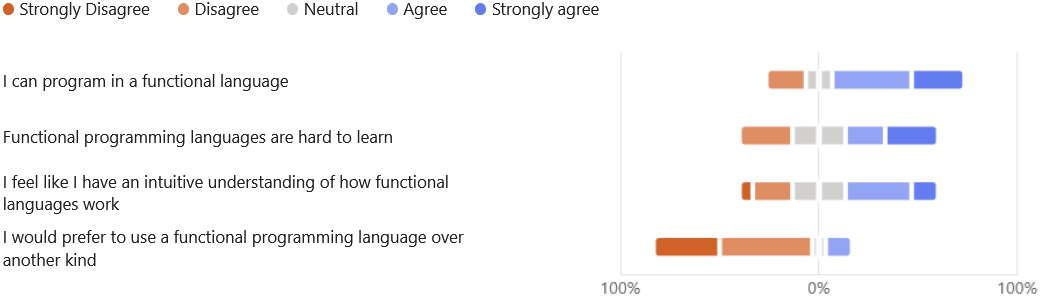
\includegraphics[width=\linewidth]{images/fp_likert.png}
%         \caption{}
%         \label{fig:fp_is_hard}
%     \end{subfigure}
%     \caption{The results of a survey performed during the testathon, where a Likert scale was used to gauge 15 participants feelings towards imperative (a) and functional (b) programming languages}
% \end{figure*}

% For imperative languages, $80\%$ of respondents agreed/strongly agreed that they can program in them, similarly $80\%$ of respondents agreed/strongly agreed that they had an intuitive understanding of them. For functional languages, $66.7\%$ of respondents strongly/agreed that they knew them, but only $47.6\%$ of respondents would agree/strongly agree that they had an intuitive understanding of them. The number of people who claim to know how to program in functional languages is less than imperative, but more striking is the difference in reported `intuition'. 

Participants were given some free-form questions:
\begin{itemize}
    \item `What do you like about the interface'
    \item `Do you have any things I can improve about the interface'
    \item `What do you like about the language'
    \item `Do you have any language features you think would make it better. I am intending to add pattern matching, so not that'
    \item `What do you like about the type system'
    \item `Anything I can improve about the type system'
\end{itemize}

The answers to these questions were mostly complimentary, but some useful information was extracted:
\begin{itemize}
    \item Participants appreciated the decluttered and simple UI. 
    \item They noticed that certain UI elements overflowed their boundaries, and that the UI had visual glitches on Safari.
    \item They found the help menu too long and wordy, and not clear or to the point enough.
    \item They liked the language, the type system and the inference. 
\end{itemize}

% I asked people who did not want to read the instructions to explain why, and their answers centred around the following points:
% \begin{itemize}
%     \item They could not find the instructions
%     \item The instructions look quite intimidating, due to being a large block of text
%     \item The instructions also look quite intimidating due to the unusual/unfamiliar pieces of syntax. This was in reference to the `Language Specification' section, and the `Types' section.
% \end{itemize}
% The first point did not provide any opportunity for further analysis, but the other points convinced me that a significant rework was needed to the UI and to the instructions menu. 

% I asked people needed further elaboration why they needed elaboration, and their answers centred around the following points:
% \begin{itemize}
%     \item The instructions contained quite a lot of `technical' language.
%     \item The instructions were not very good, and were incomplete, and often did not include new language features.
% \end{itemize}

% I could not gather data about other parts of the system, as I needed to explain the system in detail to everyone in turn, which did not allow me time to ask the questions I wanted to ask before people got bored and moved on. 

\subsubsection{Key Takeaways} The findings from the testathon informed my future testing strategy:
\begin{itemize}
    \item The `Think aloud' method of watching people interact with this version of the system and asking them to narrate what they are doing is ineffective, as the UI is not `self-explanatory' enough for people to be able to use it without help 
    \item People do not want to read things. 
\end{itemize}

Certain visual glitches were also identified and fixed in phase 2. 

\section{The Advanced Focus Group: Evaluation and Next Steps}
\label{ref:afg_figma}
\label{ref:afg}
The aims of this phase were to develop the language as well as some other more technical features of this project. To discuss the language, I held a focus group with students who were very knowledgable and interested in functional programming languages. 

This was my first of three focus groups, the most advanced of the three. As the UI/UX was not polished at this stage, I wanted to find people who would be able to discuss the parts that I had already implemented to a reasonable level of completion: the language. However, I also wanted to discuss future steps for the system as a whole. Because of this, I wanted to find people who had learned functional languages as a part of a university course fairly recently and within memory, so they would have an insight into what is required for the system to be useful for use in this setting. 

The transcript from this focus group is included in the additional submitted materials (see \ref{appx:additional_mats})

\subsection{Selection and Format}

For this focus group, I recruited four students in their fourth year of studies here at the University of Bristol. They had all taken \hyperref[COMS10016]{the first-year FP unit} 3 years prior, and they had all taken units specializing in programming language theory since, including:

\begin{itemize}
    \item The second year Programming Languages and Computation unit COMS20007, where they learnt to (among other things) `Understand the interplay between the design and implementation of programming languages' \cite{COMS20007_PLC}
    \item The third year optional Types and Lambda Calculus unit COMS30040 where they learnt (among other things): \cite{COMS30040_TLC} 
    \begin{itemize}
        \item `Type systems: types, judgements and rules'
        \item `Syntax and semantics of an untyped lambda calculus'
    \end{itemize}
    \item The fourth year optional Advanced Topics in Programming Languages, where the unit outcomes were that they should be able to (among other things): \cite{COMSM0067_ATPL}
    \begin{itemize}
        \item `Specify the dynamics of program evaluation for a variety of programming constructs'
        \item `Specify static typing rules for a variety of programming constructs'
    \end{itemize}
\end{itemize}

These people I selected for this focus group were the closest to `subject experts' that I could find while still being students. 
This focus group started with me briefly presenting SFL explorer. \ref{fig:screenshot_c2_end} shows how the system looked at this stage of the project. We also discussed the next UI iteration (see \ref{c2:next_ui}). 

\subsection{Outcomes}
Below is the summary of outcomes from the discussion with this focus groups. 

\subsubsection{The Language}
\paragraph{Positives:}
\begin{itemize}
    \item They liked the explicit match statements, and did not want me to change to more Haskell-like pattern match syntax: 
    
    `Stick with the match expressions because it's very clear that matching has happened when you have the word match there' [Participant 2, 24:11]
    \item They liked that \sflinline{Cons} was a prefix constructor rather than infix: 
    
    `I think it's good that Cons is a prefix, like a normal constructor, and not a colon or
    something like that' [Participant 4, 17:41]. 
    \item Similarly, they liked the limited set of operators, and the fact that you cannot define your own: 
    
    `I think if I was learning functional programming for the first time, I would really hope there aren't custom operators' [Participant 3, 15:56]
    
    `If I'm trying to learn functional programming, I don't think it helps me to be able to define, like, things that have different precedents. I think that distracts from learning how programs are reduced' [Participant 4, 16:42]
\end{itemize}

\paragraph{Negatives/Potential Improvements:}
\label{ref:afg_ite} 
Sentiment about the language was good, the only language specific issue was that they were confused about if-then-else syntax. They said it could be confusing to have the parser act differently for one specific function type. 

`The issue I was having is just the fact that there is a function in the prelude which has the same name as some syntactic sugar that is a parser construct' [Participant 2, 42.55]

\subsubsection{The Existing User Interface, and the System as a Whole}
\paragraph{Positives}
They really appreciated its utility for what it was designed for. Most of what we discussed was potential improvements rather than positives of the proof of concept system, however they seemed engaged and excited despite not being explicitly positive about it, beyond this one comment:
    
\begin{quotation}
\noindent `I think this is very good \ldots\ I wish I'd had this in the functional labs' [Participant 3, 1:00:09]
\end{quotation} 

\paragraph{Negatives/Potential Improvements:}
\begin{itemize}
    \item `Syntax highlighting would obviously help' [21:45]
    \item They were confused as to why, in free choice mode, some reduction options included each other: 
    
    `The first one is a chain of reductions that contains the second one. I think it's fine to display that as long as you make it visually distinct that these two are related in that way and the other reductions are just independent' [12:57]

    This could be implemented by having a dropdown where the highest level one shows all the ones below it. 

    `You could put a number next to the reduction and say, you know, this is four steps. And then \ldots make a drop-down. Yeah. So if someone wants to see what steps are going on inside there, then they could see' [08:57]
    \item They wanted an indication of which direction evaluation was going: 
    
    `Because the reduction steps generate bottom-up, it might be good to have some sort of indication about the direction things are going in' [28:12]. This was already in the new UI, which had not seen by this point in the transcript.

    \item They wanted to be able to hover over an option and have it highlight what would change: 
    
    `I think one thing that is not immediately clear is how the different reductions you see are related to the main program. If there was some way that like if you hovered over one, you could highlight the portion of the program that it corresponds to' [10:28]
\end{itemize}

\subsubsection{The Next Iteration UI Design}
\paragraph{Positives:}
\begin{itemize}
    % Make sure this stays with the prev one about reduction steps
    \item The new UI included indication of which direction evaluation was going, see above. 
    \item They liked the ability to go revert: 
    
    `Something I had not thought of, very good' [54:59]
    \item They liked the horizontal split: 
    
    `It's easier to have everything on screen and it's more akin to what people may have experienced' `Its like compiler explorer'. [52:38] `I think immediately not having to scroll is a massive plus' [52:58]
\end{itemize}

\paragraph{Negatives/Potential Improvements:}
No improvements were discussed for the next UI specifically, but most of the potential improvements for the current UI apply. 

\section{Phase 2 Conclusion}
Phase 2 resulted in a good programming language which has syntax, semantics and a type system that are fit for purpose. The language was very popular with the Testathon users as well as the Advanced Focus Group. There were no specific complaints about the language from either group. 

The proof of concept UI had mixed feedback. During the Testathon, people cited its `cleanness' i.e. lack of overcomplicating buttons. However, people did not like having to scroll to refer to the original program, and the confusing nature of the way the history was generated bottom up. The advanced focus group also had a lot of feedback on how to

The new UI as designed at the beginning of phase 2 \ref{c2:next_ui} was popular with the Advanced Focus Group. They had no specific thoughts on how to improve it, however they had many thoughts on features that could be added to the UI and the system as a whole on how to make reduction clearer. 

By the end of the project, I implemented the new UI along with syntax highlighting, and many other clarifying features. 

However, I unfortunately did not have time to work on grouping related reductions together or highlighting in source code when a progress option is hovered over what it would change, or improving the help menu. See the `future work' section \ref{conc:future_work} for more detail. 